\documentclass[10pt, compress]{beamer}

\usetheme{m}

\usepackage{booktabs}
\usepackage[scale=2]{ccicons}
\usepackage{minted}

\usepackage{graphicx} %package to manage images


\usepackage{tikz}

\usetikzlibrary{scopes}
%\documentclass[tikz, border=5pt]{standalone}
\usetikzlibrary{calc}
\usetikzlibrary{patterns}
\usepackage{tkz-euclide}
\usetkzobj{all}

\usemintedstyle{trac}

\usefonttheme[onlymath]{serif}

\newcommand\der{{\rm d}}

\title{Robot Inverse Kinematics using SQP method}
\subtitle{}
\date{\today}
\author{Xiaoqian Mu, Yuechuan Xue}
\institute{Iowa State University}

\begin{document}

\maketitle

\begin{frame}[fragile]{Problem Formulation}
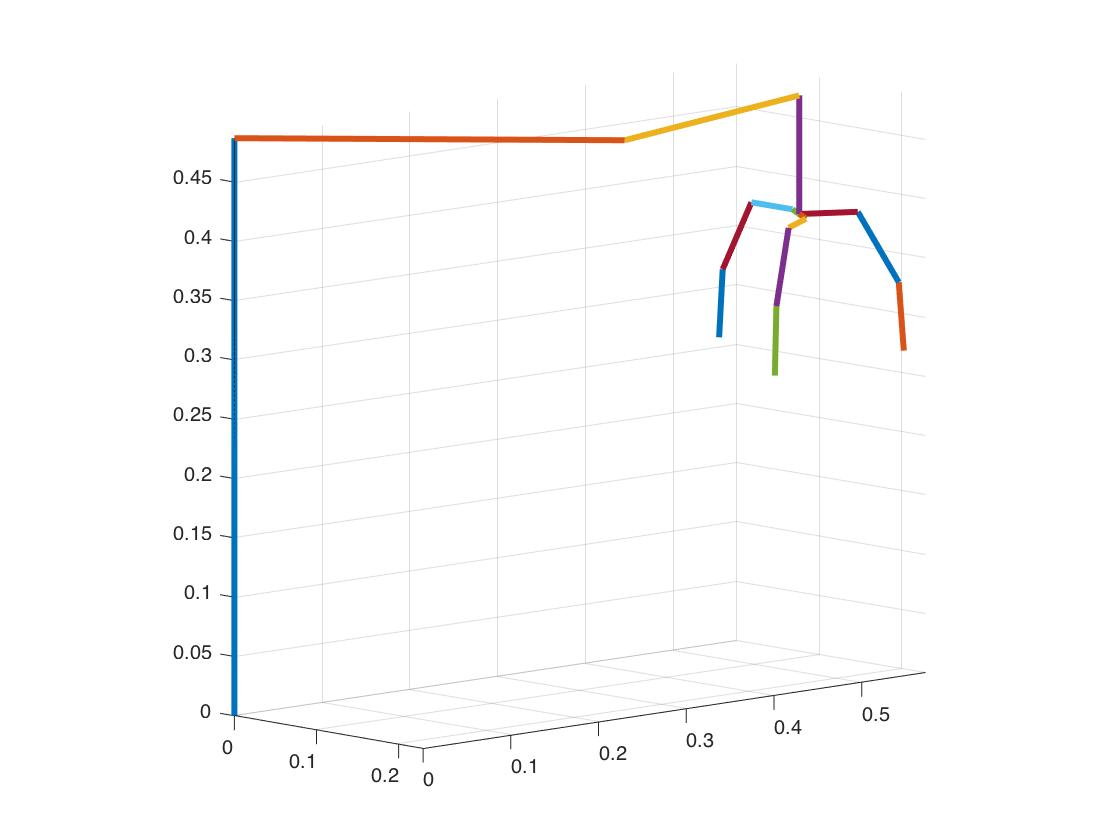
\includegraphics[width=6cm, height=4cm]{robot-matlab-config.jpg}
\end{frame}


\begin{frame}[fragile]{Rigid Motion in R$^3$}
A configuration of the system consists of the pair ($p_{ab}, R_{ab}$), and the configuration of the system if the product space of $\mathbb{R}^3$ with $SO(3)$, which shall be denoted as $SE(3)$ (for special Euclidean group):
$$SE(3) = \mathbb{R}^3 \times SO(3)$$
\end{frame}

\end{document}